\documentclass[10pt,a4paper]{article}
\usepackage{amsmath}
\usepackage{graphicx}
\title{Computing Infrastructure}
\author{Elia Ravella}
\begin{document}
	\begin{titlepage}
		\maketitle
	\end{titlepage}
	
	\tableofcontents
	\clearpage
	
	\part{Introduction}
		\section{Computing Infrastructure}
			What is a CI? A CI is a \emph{technological structure} that provides hardware and software for computation to other systems. This means a lot: is a joint (and heterogeneous) system that comprises both HW and SW to deliver a service. With CI is not intended the \emph{application delivered} but the combination of elements that makes the application available and running.\\
			So everything in between a RaspPI that does torrent seeding from a local network to the whole datacenter that runs an AWS service can be considered a computing infrastructure.
			
	\part{Hardware Infrastructures}
		\section{Data Centers}
			\subsection{Pros and cons}
				Data centers are big centralized CIs that comprise a lot of servers (to provide computations) a communication infrastructure, and a storage service.\\ 
				PROS of a DC:
				\begin{itemize}
					\item Lower IT cost: renting a virtual machine is cheaper than buying / building and maintaining a whole system (for some time horizons, of course);
					\item High performance: virtualized resources make scaling easier, and provides optimized and finely tuned services that an in-house solution cannot provide \emph{so} easily and fast;
					\item No effort software updates;
					\item Unlimited (!) storage capacity;
					\item Increased data reliability;
					\item Universality of accesses;
					\item Device indipendence.
				\end{itemize}
				The CONS of a DC can be found simply inverting the POV for the PROS aspects: outsourcing resources gives "someone else" the control over some crucial aspects of a CI. This is a good thing when costs (also time costs) must be reduced, but can be a bad thing when a fine grained control over a full system is needed. Also, \emph{latency} pops in, due to the needed connection to the DC.
				
			\subsection{DCs ans WSCs}
				The data center approach has been emerging in the last years. The idea behind it is that we should not "overpack" nodes of a network with all the computing capabilities required, but instead giving them a connection to such CIs. Data centers are the perfect example for this paradigm: the user interact with a client (that can be \emph{any kind of device}) that also interact with a remote structure to provide computations. To a careful watch, SaaS and their spread are a direct conseguence of this paradigm shift. Another use of DCs is using their computing capabilities not in a fragmented way to provide miriads of services, but to perform an \emph{extremely costly computation}, like a training of a neural network.\\
				From a DC approach we are moving to a Warehouse Scale Computers nowadays. This latter approach consists of NOT "mix up the pot" in a DC (so having a lot of heterogeneous technologies in order to achieve different tasks) but instead to "homogeneify" the cloud structure in order to do better optimization of it. Not only in the HW, but also in the SW. To centralize the DC capabilities under a single organization (as often happens) means that clients no more run their application on someone else's hardware, but instead choose from a set of precooked solutions by such vendor/organization. Is this \emph{bad}? WSCs are just a "SaaS - oriented" Data Center Architectures, so \emph{there's no real transition between DCs and WCSs} the only transition is in the number of \emph{virtualiazed layers the client must go through to access and application}.\\
				We can sum up the difference between DCs and WSCs in this way: where DCs are intended as a powerful collection of different servers, WSCs tries to offer a homogeneous interface that can be used also as a single server to such a collection of hardware. Still, if we consider a lerger definition for DCs, WSCs are a type of DCs. 
				
			\subsection{Architectural Overview of DCs and WCSs}
				A standard data center building is organized in separated modules, every one dedicated to a specific task. The four main modules types are
				\begin{itemize}
					\item Servers: computations
					\item Storage
					\item Networking: intended as the whole communication infrastructure
					\item Building-integrated systems:
						\begin{itemize}
							\item Cooling system: often as powerful as the server themselves, fundamental for getting rid of excess heat
							\item Power supply: integrated in the building and provided with systems to avoid power shortage
							\item Failure recovery: physically realized as a building module in order to be as most fault - tolerant
						\end{itemize}
				\end{itemize}
				Servers are organized in racks, blades or tower, and are the classical computational unit usually found in server farms. They could also not have memory attached.\\
				Storage is the crucial long term memory for a CI. Usually built with flash SSDs and ferromgnetic mechanical disks. The memory units must provide high speed I/O capabilities, and also advanced networking power, also at software level (NAS, SAN, DAS).\\
				The networking infrastructure is the backbone of the communication in (and from/to) a data center. Structured hierarchical approach to networking structures and organization are used to ensure security and performace\\
				The building itself is part of the CI.\\
				Next sections will delve into the details of the single modules.
			
			\subsection{Servers}
				Servers are the computational compartment of a WSC. They're organized in racks (shelves) that host the computational units (pizza box computer). Servers are just computers. That's all. They got a MOBO, local primary memory, a CPU, and I/O capabilities. They can be organized as
				\begin{itemize}
					\item Towers: cheap, cooling is easy, upgrade is easy. They're also big, and they provide low density of computational power.
					\item Blades: also called hybrid racks, the idea is similar to the rack system, but a server is inserted \emph{vertically} instead of \emph{horizontally} in a dedicated place. This (together with the average smaller size of a blade server) enhances computation per volume ratio while keeping all the pros of a rack system. Blade servers have disadvantages: heat management is complex, and enclosures and envelops are more expensive wrt racks.
					\item Racks: literal racks that host the pizza box shaped computational units, and accomodate all the wiring and additional connection or cooling systems. They can host also heterogeneus components, not only standard computational modules. Rack's dimension and geometry is a standard. Rack organization provides better failure handling and simplified cable management, but they're more power demanding (wrt towers) and mainteinance is a mess (mmultiple devices must be maintained at the same time).
				\end{itemize}
				
				\subsubsection{Hardware Accellerator}
					WSCs architectures and the rise of heavy computation loads (like for intense machine learning and AI training) have caused a spike in the complexity required every computation, even far beyond the Moore's law. To satisfy this need, dedicated hardware (in the form of \emph{hardware accellerators}) are deployed in WSCs, to enhance the performance in determined fields.
					
					\paragraph{GPU}
						Graphical Processing Units are featured in accellerators to enhance \emph{parallel fast computation}. Due to the archiecture of them, they're also perfect to do matrix computation. 
						
					\paragraph{TPU}
						Tensor Processing Units. These are more specialized GPUs in the machine learning direction. They're (simplifiyng) custom circuits to support tensor computations (matrix calculus) that are \emph{very fast} at doing so. 
						
					\paragraph{FPGA}
						Good ol' Field Programmable Gate Array circuits are still used to enhance performance in custom computational oriented architectures (apple afterburner...). These circuits are somewhat "fully customizable" hardware computers that if programmed in a very specific way can enhance \emph{every kind} of possible computation. 
			
			\subsection{Storage}
				Storage. Not much more. Technologies involved: HDDs and SSDs and Flash memory. Performance (and relevant) parameters:
				\begin{itemize}
					\item read / write speed and latency (or seek time)
					\item memory density
					\item security: but this is intended as an hardware security, not data security (for now)
					\item cost
				\end{itemize}
				
				\subsubsection{Storage Systems - DAS, NAS, SAN}
					\begin{itemize}
						\item Direct Attached Storage is every device that offers storage capabilities and is directly attached to the unit processing such data in the storage. HDDs are DAS for personal computers, for example. They're directly accessible from the OS of the machine accessing it.
						\item Network Attached Storage is a storage system that lies \emph{on the other end} of a network. A NAS only offers data services accessible from dedicated protocols (as FTP, SAMBA) and it's \emph{an actual computer} that offers services.
						\item Storage Area Network is like NAS, but the remote storage unit are \emph{passive} and are directly accessible by the OS (by means still of a network connection). They're \emph{remotely accessed simple storage devices}.
					\end{itemize}
					\begin{figure}
						\centering
						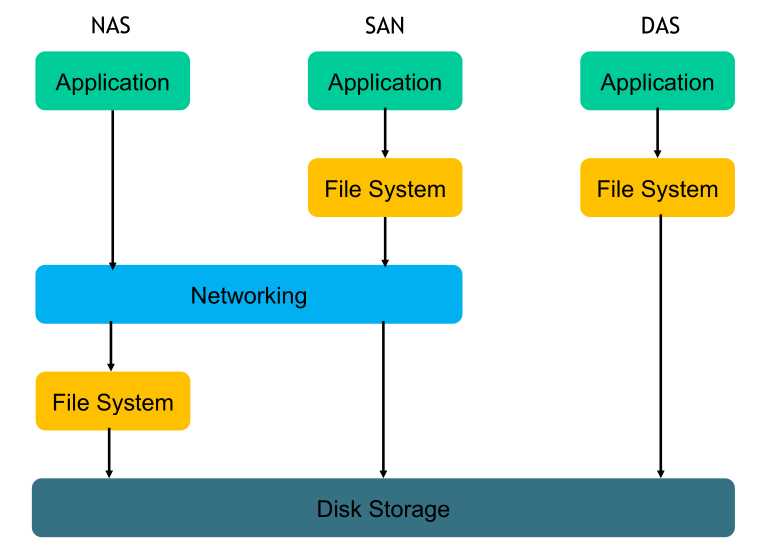
\includegraphics[width = \textwidth]{./images/storage.png}
					\end{figure}
					
					\paragraph{DAS}
						Traditional attached local storage systems. They're difficult to scale. They are difficult to manage when particular storage solutions are needed. Moreover, the OS's proprietary file sharing model / protocol / software must be used in order to share files.
						
					\paragraph{NAS}
						A NAS is a \emph{full fledged computer} that's \emph{only meant for storage services}, accessible through network protocols. It's located somewhere in the network. It's easily scalable (both augmenting the storage of a single NAS or multiplying the NAS number work).
					
					\paragraph{SAN}
						Disks are visible \emph{like local storage, like DAS} to the server machina, but they're network attached. They have specialize hardware that mask the network in between, and the SAN can be accessed \emph{directly through the filesystem}. 
				
			\subsection{Networking}
				A WSC networking system can be divided in 2 separate blocks:
				\begin{itemize}
					\item an internal LAN that connects all the components (the servers) among themselves
					\item an interface to the internet (DMZ..?)
				\end{itemize}
				
				Obviously, the networking infrastructure in a WSC is crucial because it also connects the functional units (as the server) to the storage infrastructure and so it's \emph{fundamental} that this connections is solid. The need of inter-server bandwidth incerases exponentially with the number of server, obviously.\\
				A WSC internal network is usually divided in 3 levels:
				\begin{enumerate}
					\item Access: this network layer is the one that connects the servers to the network. It's embodied by the network infrastructures embedded in the server racks.
					\item Aggregation: this level groups the servers together (VLAN-like) and it's usually implemented as Top Of the Rack switches, that group together all the server in a aisle (for example).
					\item Core: furthest level from the single server, aggregates entities of the "aggregation" level.
				\end{enumerate}
				
			\subsection{Building and Non-IT Equipment}
				The way in which the hardware is arranged \emph{inside} a DC is as crucial as the building composing the DC itself, as well as the non-IT instruments (like the cooling system, or the enrgy system) that completes the DC structure.\\
				
				
			
	\part{Software Infrastructure}
	
	\part{Methods}
		\section{HDD and RAID Technologies}
			Memory and files in disks are organized in clusters to simplify the management of the data. We have:
			\begin{equation}
				\begin{cases}
					a = \text{ actual size of a file on disk}\\
					c = \text{ cluster size}\\
					s = \text{ file size}
				\end{cases}
			\end{equation}
			and it holds that $ a = ceiling(\frac{s}{c}) \,\times\, c$.
			
			\subsection{Data and Metadata}
				Data is the content stored in a mass storage device. Metadata is (as the name suggests) additional data stored in the storage device \emph{that not contains actual content}. Metadata contains indexes, addresses, cached data that is used to manage \emph{the actual data stored}.
				
			\subsection{Magnetic Hard Drives}
				Magnetic disks have an internal structure and an external interface to manage files and data. The internal structure is often based in c/h/s coordinates, that are cylinder, head and sector locations. The external interface is usually composed of clusters. The traslation is carried out directly by the electronics on the disk.
				
				\subsubsection{Delays}
					The principles on which the HDD storage is based relies on some phisical objects and their movement. The intrinsic limits of this system translates into delays in the reading of data. Four type of delays can be identified:
					\begin{itemize}
						\item Rotational: it's the time occurred to move the portion of plate under the desired head. It's related to RPM, of course
						\item Seek: it's the time needed to a head to move from a track to another
						\item Transfer: actual time to read the bytes
						\item Control: overhead time, related to the circuitery that manages the hardware
					\end{itemize}
					
					So, in order to calculate the actual time that passes between the issue of the read command to the presence of the desidered file on the I/O bus we have to sum all the delays.
					\begin{equation}
						T_{read} = T_{rotate} + T_{seek} + T_{transfer} + T_{overhead}
					\end{equation}
					Usually, the transfer speed is usually given as transfer ratio $\frac{MB}{sec}$. 
					
					\paragraph{Reducing Latency}
						Caching is the most used mechanism to make data available \emph{faster} in order to reduce latency. Usually, at hardware level, the cache is implemented by means of a phisycal additional RAM memory built directly in the HDD.
						
						\subparagraph{Read Cache}
							Often accessed data access can be reduced if there's no need to go down to the plate in order to read it all the times.
						
						\subparagraph{Write Back Cache}
							Write buffer: writes are cached before accessing the disk, and then flushed at the end. N.B.: the "write finish" signal is issued at the end of the \emph{caching} of the data.
							
						\subparagraph{Write Through Cache}
							No write buffer: the "write finish" signal is issued after the write is actual written on the disk.
							
						\subparagraph{Scheduling}
							As always, reordering operation in order to maximize efficency is a solid approach to enhance performance, in this case reducing latency in accessing the disk. These kind of approaches (that usually prefers "near" sector) are prone to starvation, usually. Workaround to starvation problem usually are based on linearizing the traversing of the cylinders, like the elevator meachanism.\\
			
			\subsection{RAID}
				Redundant Array of Inexpensive Disks is a technology that exploits the parallelization of I/O bus to multiple disks in order to enhance security, write and read speed, and fault tolerance. Data are copied / distributed on multiple disks, that are presented to the OS as a single one. Different strategies can be put in place to organize the data pieces:
				\begin{enumerate}
					\item data striping: in a round robin fashion, data are partitioned circularly in the disk. This means that each file, when it's written, it's stripped down to fixed dimension blocks and then memorized in different disks. This enhance write and read speed: we can exploit parallel write/read operation. This also increase fault probability (more disks = more fault) decreasing reliability.
				\end{enumerate}
							
	
	\part{Dependability}
		\section{Probabilistic approach}
			Dependability represents the \emph{availability performance} of a system. It encompasses 
			\begin{itemize}
				\item Reliability
				\item Availability
				\item Maintainability
			\end{itemize}
			
			Dependability is approached with a statistical/probabilistic POV due to the high human component in it.\\
			Two functions describes the system: F(t) and f(t), respectively the cumulative function and the fault probabilistic distribution. The former represents the \emph{unreliability} of the system analyzed. So, we can define $R(t) =  1 - F(t)$ as the reliability function.\\
			Probabilistics recall:

			\begin{align}
				f(t) \rightarrow \text{ probabilistic distribution}\\
				F(t) = \int_{0}^{t}f(t)dt \rightarrow \text{ cumulative function, unreliability}\\
				R(t) = 1 - F(t) \rightarrow \text{ reliability function}
			\end{align}

			To be noticed: the function $F(t_i)$ represents the probability that component $i$ is working at time $t_i$ \emph{knowing it was working at time 0}. This is to be taken in mind to make a comparison with the failure rate.\\
			From this we can define the Mean Time To Failure for a component (that's the expected value):
			\begin{equation}
				\begin{cases}
					MTTF = \int_0^{\infty}t \cdot f(t)dt\\
					MTTF = \int_0^{\infty}R(t)dt
				\end{cases}
			\end{equation}
			We can also define the failure rate (mathematically, the conditioned probability):
			\begin{equation}
				\lambda(t)dt = F(t < T \leq t+dt \,\vert\, T > t)
			\end{equation}
			So the failure rate represents the probability of failure \emph{assuming the component was working the instant before}. This function can be seen as the number of failures in a given interval.
			
			\subsection{Failure Rate}
				Type of malfuntioning:
				\begin{itemize}
					\item Fault: physical defect or software bugs.
					\item Error: program incorrectness that can result from a fault.
					\item Failure: nonperformance of some actions that were expected. They can be result of an error.
				\end{itemize}
				
				\paragraph{Properties of the failure rate}
					Probabilistically, failure rate is
					\begin{equation}
						\lambda(t)dt = F(t < T \leq t+dt \,\vert\, T > t)
					\end{equation}
					So we can derive
					\begin{equation}
						\lambda(t)dt = \frac{P(t < T < t + dt \cap T > t)}{P(T > t)}
					\end{equation}
					From the definition of combined probability, with P as probability. Given
					\begin{equation}
						P(t < T < t+dt) \cap P(T > t) = P(t < T < t+dt)
					\end{equation}
					We obtain
					\begin{equation}
						\lambda(t)dt = \frac{f(t)dt}{R(t)} = \frac{dF(t)}{R(t)} = -\frac{dR(t)}{R(t)}
					\end{equation}
				
				\paragraph{Reliability as Weibull}
					Failure rate $\lambda(t)$ function has a peculiar function shape: a \emph{bathub} (or long U) shape. The failure rate is high in the starting period and decreases (infant mortality effect) to the costant level during the useful lifetime (costant probability of failures) and it raises again at the end (wear out period).\\
					
					In fact, reliability follows the \emph{Weibull distribution} so definied: $y(x) = e^{-(\frac{x}{\alpha})^{\beta}}$. So (due to the $\lambda(t) = f(t) / R(t)$ relation) we obtain
					\begin{equation}
						\lambda(t) = \frac{\beta}{\alpha}(\frac{t}{\alpha})^{\beta - 1}
					\end{equation}
					
				\paragraph{Reliability as exponential}
					We can also model the reliability as an exponential function (so $R(t) = e^{-\lambda t}$) we than obtain
					\begin{equation}
						\begin{cases}
							F(t) = 1 - e^{-\lambda t} \\
							f(t) = \lambda e^{-\lambda t} \\
							MTTF = \int_{0}^{\infty} t\cdot \lambda e^{-\lambda t} dt = \frac{1}{\lambda}\\
						\end{cases}
					\end{equation}
					So we can express the reliability as function of MTTF: $R(t) = e^{-\frac{t}{MTTF}}$. And we all know that in certain conditions (like $\frac{t}{MTTF} << 1$) an exponential function can be approximated to a linear function.

			\subsection{System level reliability}
				We can model the system relibility mainly with RBDs: Reliability Block Diagram. These simply outline the operational dependency between components. The main assumption of the RBD is that the failures are \emph{indipendent}, that implies that are no "cascading failures".\\
				It's easy to calculate the overall reliability:
				\begin{equation}
					\begin{cases}
						\text{Serial components: } R_s(t) = \prod_{i=1}^{n}R_i(t)\\
						\text{Parallel components: } R_p(t) = 1 - \prod_{i=1}^{n} (1-R_i(t))
					\end{cases}
				\end{equation}
				The MTTF is also altered from the serialization or parallelization of components. In particular, in a serie with n identical components, $MTTF_{serie} = \frac{MTTF}{n}$. The general formula is the one used for parallel resistors:
				\begin{equation}
					MTTF_{serie} = \frac{1}{\sum_{i=1}^{n}(\frac{1}{MTTF_i})}
				\end{equation}
				For parallel system, things get complicated. The MTTF is calculated from the unreliability, integrating between 0 and $\infty$. The resulting formula is
				\begin{equation}
					MTTF_{parallel} = \sum_{i=1}^{n}(MTTF_i) - \frac{1}{\sum_{i=1}^{n}(\frac{1}{MTTF_i})}
				\end{equation}
				Notice that the second term of that sum is exactly $MTTF_{serie}$ of that configuration. Again, the formula can be simplified if the components are identical: $MTTF_{parallel identical} = MTTF_i*(\sum_{i=1}^{n-1}(\frac{1}{n-i}))$\\
				
				\paragraph{Extension of MTTF calculation to complex systems}
					We can apply the calculation of the \emph{reliability} of a complex systems directly with the formulas, but the same cannot be done with MTTF. This is due to the fact that a complex system has not anymore a simple failure rate distribution, and this messes up the MTTF calculation, that's an integral on that function. So, I must pass through the reliability calculation.

			\subsection{Availability}
				Introducing MTTR, Mean Time To Repair. This represents the average time required to replace a failed component and "bring the system back up" after a failure. It can be the restart time (for software module) or the replace time (for an hardware component).\\
				Another interval to be taken into consideration when talking about availability is the Mean Time Between Failure, that's just the sum of $MTTF + MTTR$. Availability is defined as the probability of a system to be up and running at a given istant. So $Av = \frac{MTTF}{MTBF}$ that corresponds to
				\begin{equation}
					Availability = \frac{MTTF}{MTTF+MTTR}
				\end{equation}
				The slight difference between availability and reliability takes into consideration the repairing of a system in the case it goes down. The availability function is calculated with \emph{the same identical formulas} used to calculate the reliability for parallel and serial components.\\
				Talking about MTTF when taking into consideration that components can be \emph{repaired} must be carefully handled: for example, if a parallel system has \emph{interleaving} failures, it never fails enitrely. A way of calculating MTTF for repairable system consists in inverting formula (9), obtaining
				\begin{equation}
					MTTF = \frac{Av*MTTR}{1-Av}
				\end{equation}









\end{document}
